\documentclass{beamer}
\usetheme{CambridgeUS}
\usefonttheme{serif}
\usecolortheme{default}
\usepackage[T1]{fontenc}
\usepackage[utf8]{inputenc}
\usepackage{fixltx2e}
\usepackage{siunitx}
\usepackage{graphicx}
\usepackage{svg}
\usepackage{csquotes}
\usepackage{simpler-wick}
\usepackage{appendix} 
\usepackage{longtable}
%\usepackage[ddmmyyyy]{datetime}
\usepackage{float}
\usepackage{wrapfig}
\usepackage{rotating}
\usepackage[normalem]{ulem}
\usepackage{slashed}
\usepackage{amsmath}
\usepackage{textcomp}
\usepackage{marvosym}

\usepackage{wasysym}
\usepackage{amssymb}
\usepackage{tikz}
\usepackage{multirow}
\usepackage{pdfpages}
\usepackage{tabu}
\usepackage{hyperref}
\graphicspath{ {./img/} }
\tolerance=1000
\usepackage[spanish,es-tabla,es-nodecimaldot]{babel}
\uselanguage{Spanish}
\languagepath{Spanish}
\deftranslation[to=Spanish]{Lemma}{Lema}
\usepackage{gensymb}
\usepackage{wasysym}
\usepackage{subcaption}
\usepackage{braket}
\usepackage{amsthm}
\usepackage{mathtools}
\usepackage[backend=biber]{biblatex}
\usepackage[font=small,labelfont=bf]{caption}
\usepackage{circuitikz}
\usepackage{cancel}
\usepackage{minted}
\usepackage{movie15}
\usepackage{ragged2e}   %new code
\addtobeamertemplate{block begin}{}{\justifying}  %new code
\apptocmd{\frame}{}{\justifying}{}
\addtobeamertemplate{block example begin}{}{\justifying}  %new code
\addtobeamertemplate{block alert begin}{}{\justifying}  %new code



\renewcommand{\appendixname}{Anexos}
\renewcommand{\appendixtocname}{Anexos}
\renewcommand{\appendixpagename}{Anexos}
\newcommand{\rcor}{\right\rbrace}
\newcommand{\lcor}{\left\lbrace }
\newcommand{\comen}{\textbf{Comentarios:}}

\title[Trabajo de fin de master]{Separación de cascadas electromagnéticas en el experimento SBND mediante técnicas de Machine Learning}
\subtitle[]{}
\author[Alejandro P. M.]{Alejandro Ponce Miguela\\
$~$\\
Tutores: Alberto Guillén Perales y Bruno Zamorano García}
\institute[Univ. de Granada]{Universidad de Granada}
\date{}

\hypersetup{
  pdfkeywords={},
  pdfsubject={},
  pdfcreator={Alejandro Ponce Miguela}}
\newtheorem{teor}{Teorema}
\newtheorem{defi}{Definición}
\newtheorem{lema}{Lema}
\newtheorem{ejem}{Ejemplo}[subsection]

\renewcommand\qedsymbol{$\blacksquare$}


\begin{document}
\frame{\titlepage}
\begin{frame}
  \begin{figure}[h!]
    \centering
        
\includegraphics[scale=0.19]{dalle.jpg} 
        \caption{Un astronauta jugando al baloncesto con gatos en el espacio con un estilo minimalista. \url{https://openai.com/dall-e-2/\#demos}.}
\end{figure}

\end{frame}

\begin{frame}
  \frametitle{Índice}
  \tableofcontents
\end{frame}


\section{Objetivos}
\begin{frame}
  \frametitle{Objetivos}
  \begin{itemize}
    \item Aprender la física necesaria para la resolución del problema.
    \item Aprender técnica de MLOps.
    \item Usar Pytorch para el diseño de los modelos de DL.
    \item Lograr la clasificación de cascadas electromagnéticas.
  \end{itemize}
%   \begin{figure}[h!]
%     \centering
%     \begin{subfigure}[]{0.49\textwidth}
%         \centering
%         
\includegraphics[scale=0.13]{copo.png} 
%     \end{subfigure}
%     \begin{subfigure}[]{0.49\textwidth}
%         \centering
%         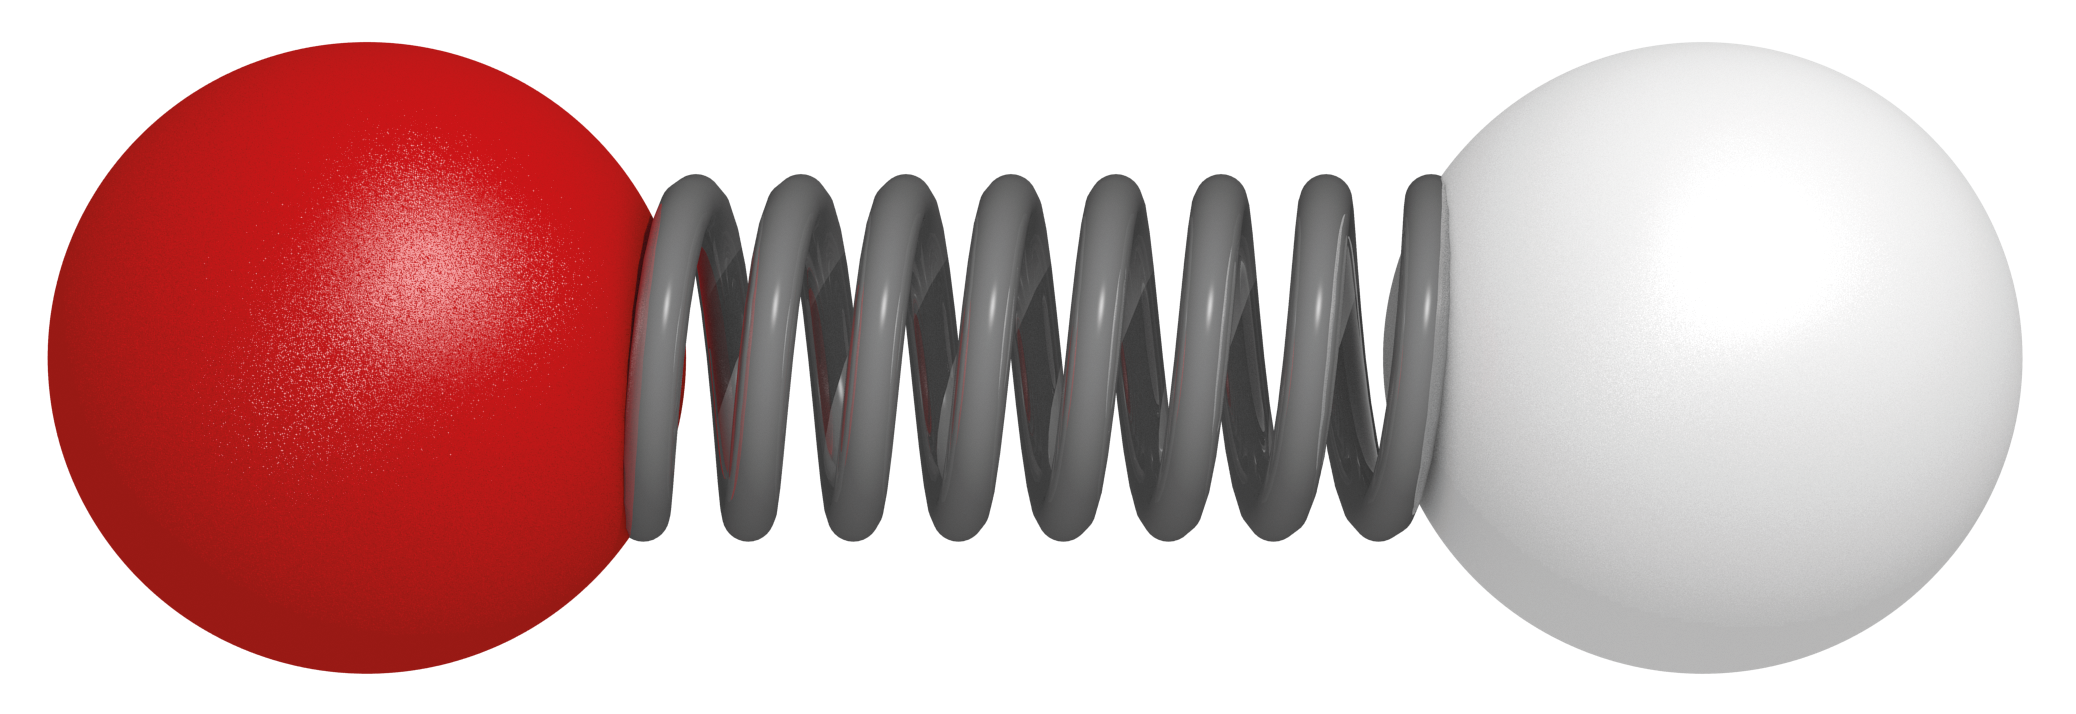
\includegraphics[scale=0.27]{molecula.png}
%     \end{subfigure}
% \end{figure}
% \url{https://toppng.com/snowflake-vector-PNG-free-PNG-Images_77960}
\end{frame}

        % \includemovie[autoplay]{0.9\textwidth}{0.9\textheight}{cutVFinal.mp4}

\section{Contextualización física}
\begin{frame}
  \frametitle{Neutrino estéril}
  \begin{figure}
    \centering
        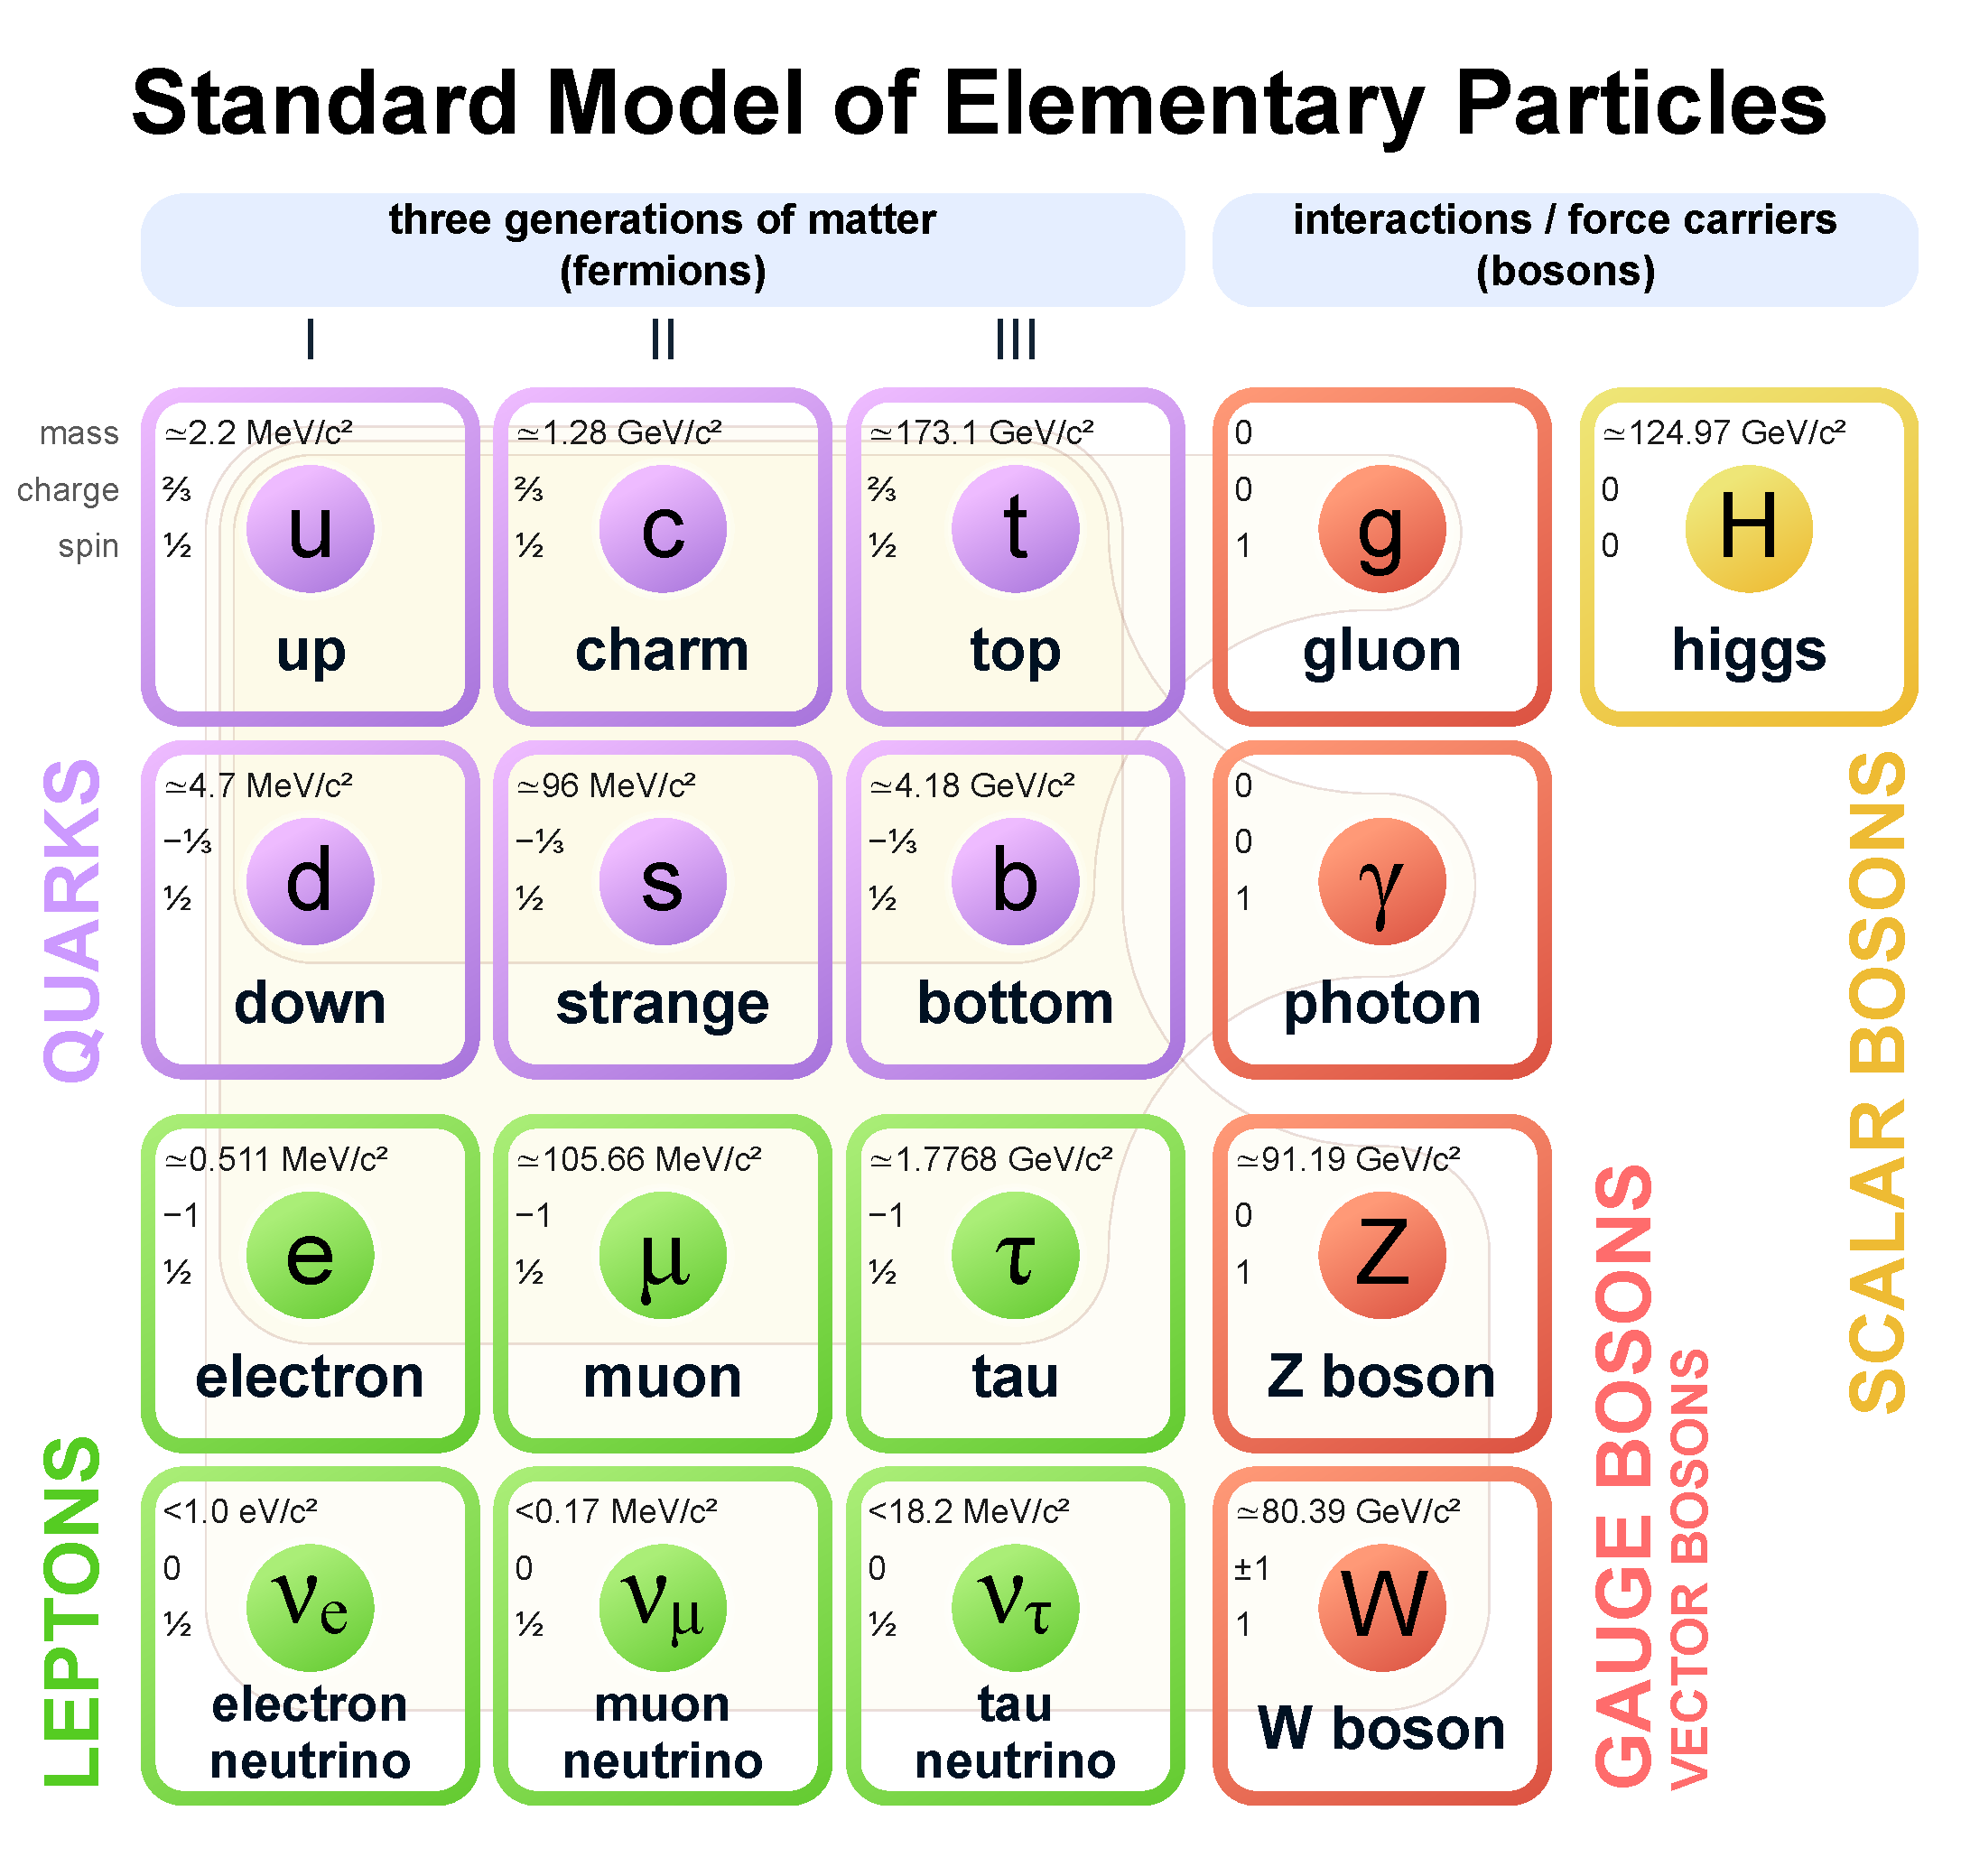
\includegraphics[scale=0.17]{Standard_Model_of_Elementary_Particles.pdf} 
  \end{figure}
  \url{https://en.wikipedia.org/wiki/File:Standard_Model_of_Elementary_Particles.svg}
\end{frame}
\begin{frame}
  \frametitle{Detección de neutrinos}
  \begin{itemize}
    \item Muy complicada debido a la poca interacción con la materia.
    \item Detectores LArTPC: SBND y DUNE.
    \item Neutrinos electrónico dan lugar a cascadas electromagnéticas. 
  \end{itemize}
  \begin{figure}
    \centering
        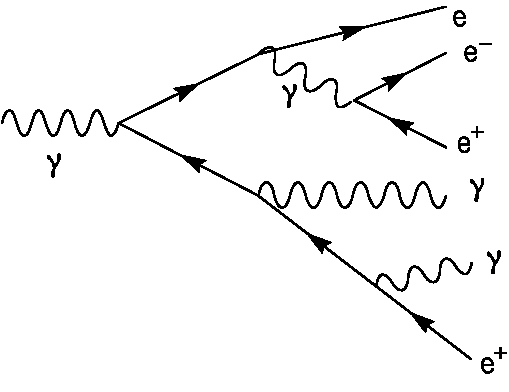
\includegraphics[scale=0.5]{Schematic_of_a_particle_shower.pdf} 
  \end{figure}
  \url{https://en.wikipedia.org/wiki/File:schematic_of_a_particle_shower.svg}
\end{frame}
\begin{frame}
  \frametitle{LArTPC}
    \begin{figure}
      \centering
      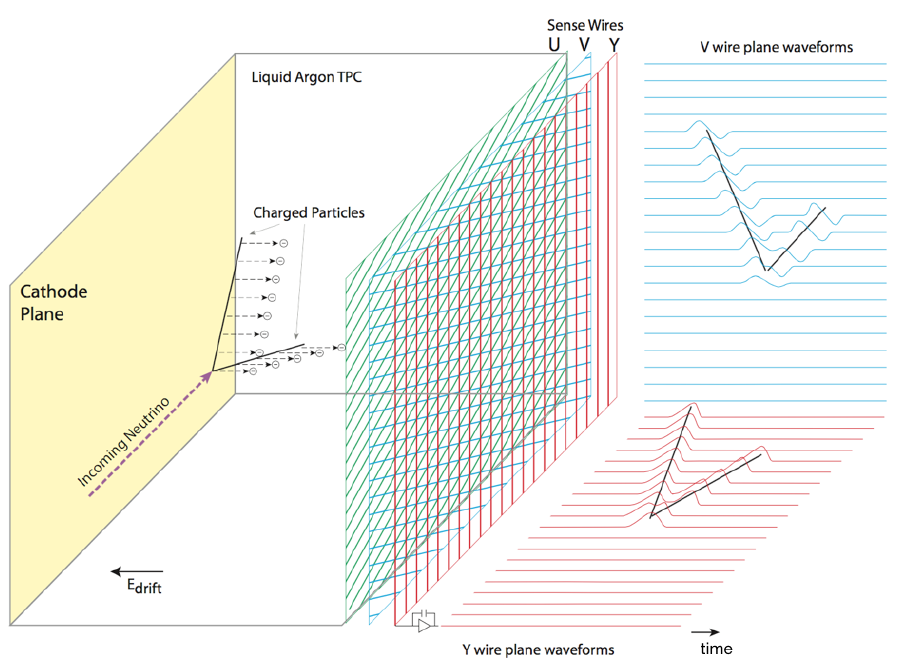
\includegraphics[scale=0.5]{planos_sensado.PNG}
    \end{figure}
\end{frame}

\begin{frame}
  \frametitle{Resumen}
  Pensar
\end{frame}

\section{Estudio de los datos: Representaciones propuestas}
\begin{frame}
  \frametitle{Datos}
  mencionar forma y que vamos a usar CNN, es una elección
\end{frame}
\begin{frame}
  \frametitle{Creación de las imágenes}
  comentar que discretizamos poner figura
\end{frame}
\begin{frame}
  \frametitle{Representación tridimensional}
\end{frame}
\begin{frame}
  \frametitle{Proyección de un eje}
\end{frame}
\begin{frame}
  \frametitle{Proyección de un eje con color}
\end{frame}
\begin{frame}
  \frametitle{Transformers}
  SOLO SI TIEMPO
\end{frame}
\begin{frame}
  \frametitle{Modelos}
\end{frame}
\section{Resultados}
\begin{frame}
  \frametitle{Selección de resolución y representación}
  mencionar que la 3d mal pero hay alternativas
\end{frame}
\begin{frame}
  \frametitle{Ajuste de hiperparámetros}
\end{frame}
\begin{frame}
  \frametitle{Estudio del mejor modelo}
\end{frame}
\begin{frame}
  \frametitle{Agregación de modelos}
\end{frame}
\section{Conclusiones}
\begin{frame}
  \frametitle{Conclusiones}
  \begin{itemize}
    \item Poner en manifiesto la utilidad de la teoría de grupos:
    \begin{itemize}
      \item Descripción matemática de la \textbf{simetría} y la \textbf{degeneración}.
      \item \textbf{Caracterización de estados}.
    \end{itemize}
    \item Descripción de \textbf{moléculas diatómicas} usando el hamiltoniano del oscilador armónico con interacción a dos cuerpos.
    \item Se pude \textbf{mejorar} el ajuste si incluimos \textbf{invariantes de Casimir} de orden superior en el limite $SO(2)$.
    \item Establece las bases para el estudio de \textbf{moléculas más complejas}. Moléculas triatómicas usando el $U(2)\otimes U(2)$.
    \item Mejora en mis conocimientos en Python y en el uso de ordenadores para la resolución de problemas físicos.
  \end{itemize}

\end{frame}

\begin{frame}
  \frametitle{Diagonalización del hamiltoniano}
  \begin{equation*}
    \hat{H} = E_0' + \epsilon\hat{n}_t + \alpha\hat{n}_t^2 + \beta\hat{J}_z^2.
  \end{equation*}
  Base $\ket{[N]n_t}$:
    \begin{equation*}
      \bra{jm'}\hat{H}\ket{jm}, \quad m,m' = -j,-j+1\dots, j.
  \end{equation*}
  Necesitamos obtener:
  \begin{equation*}
    \begin{split}
    \hat{n}_t\ket{jm} &= \frac{N}{2}\ket{jm} +\\
    &- \frac{1}{2}\sqrt{j\left(j+1\right)-m\left(m + 1\right)}\ket{jm+1}+\\
    &- \frac{1}{2}\sqrt{j\left(j+1\right)-m\left(m - 1\right)}\ket{jm-1}.
\end{split}
\end{equation*}
\end{frame}
\begin{frame}
  \frametitle{Resultados}
  \begin{itemize}
    \item Molécula HCl:
    \begin{table}[h!]
      \centering
      \begin{tabular}{|c|c|c|}
      \hline
                          & $\omega_e \hbar$ (cm$^{-1}$) & $x_e\omega_e \hbar$ (cm$^{-1}$) \\ \hline
      Experimental &     2988.90                         &   51.60                               \\ \hline
      Modelo              & 2988.90                             & 51.60                                    \\ \hline
      \end{tabular}
  \end{table}
    \item Molécula O$_2$:
    \begin{table}[t]
      \centering
      \begin{tabular}{|c|c|c|}
      \hline
                          & $\omega_e \hbar$ (cm$^{-1}$) & $x_e\omega_e \hbar$ (cm$^{-1}$)\\ \hline
      Experimental &     1580.361                         &   12.0730 \\ \hline
      Modelo              & 1580.284                             & 11.5978\\ \hline
      \end{tabular}
  \end{table}
  \end{itemize}
\end{frame}

\end{document}